\section{Deployment Diagram} \hypertarget{section::\theHsection}
Il deployment diagram mostrato nella Figura 5.1 del sistema evidenzia quali dispositivi vengono considerati, le interconnessioni tra loro e dove le componenti software verranno istanziate.

Nel nostro caso abbiamo 4 "device":\\
Un device è rappresentato dal Client che tramite protocollo http invia una richeista al device Server, esso al suo interno presenta una componente Web Browser che si interfaccerà con il Server.

Sono presenti due device di supporto alla nostra applicazione: Open Charge Map Server e Open Street Map Server queste due componenti restituiscono tramite una richiesta di tipo REST la posizione delle colonnine e il percorso da un punto di partenza ad un punto di destinazione richiesto dall'utente.
Il cuore del nostro software è presente dentro il device Server in cui sono presenti 5 componenti. Il componente charger\textunderscore location\textunderscore data\textunderscore feeder si occupa di scaricare le colonnine tramite l'API di Open Charge Map e le passa al modulo general\textunderscore data\textunderscore bank che contiene i metodi atti a generare la struttura dati che svolgerà il ruolo di database locale. itinerary\textunderscore feeder è il modulo che calcola il percorso attraverso l'API di Open Street Map. Il componente algorithm\textunderscore calculation incorpora l'algoritmo che si occuperà di trovare le colonnine a cui fermarsi. Infine client\textunderscore communication si occupa di ricevere gli input dall'utente e di restituire il risultato a schermo. 



\begin{figure}[htp]
\centering
{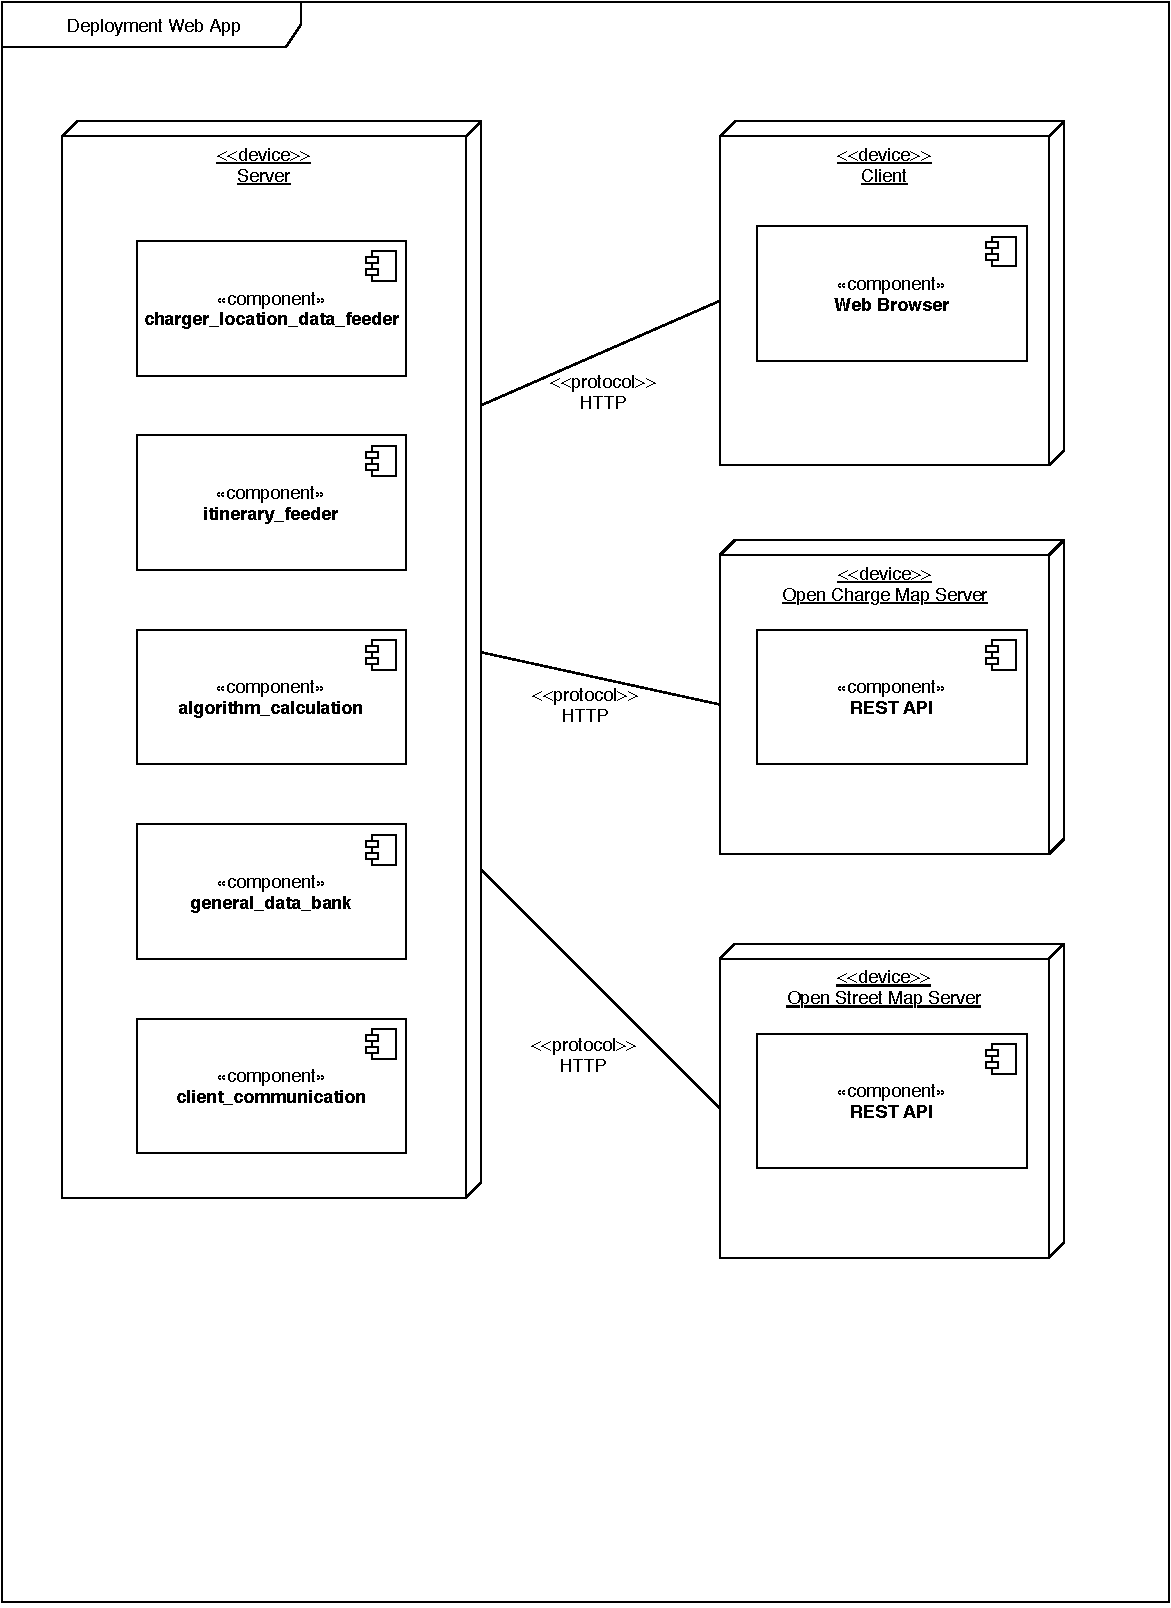
\includegraphics[scale=0.6]{Immagini/Deployment_Diagram.pdf}}
\caption{Deployment Diagram}
\end{figure}

\subsection{Architettura Hardware}

L'architettura che è emersa è ti tipo client-server a 2 livelli. Nel primo livello il client è impersonato dall'utilizzatore finale che richiede un servizio al nostro server attraverso il protocollo http. Nel secondo livello il nostro server recita la parte del client, richiedendo dei servizi alle due API a cui ci appoggiamo. (Figura 5.2 e Figura 5.3) \autocite[\protect\label{BassClementsKazman}][]{BassClementsKazman}

\begin{figure}[htp]
\centering
{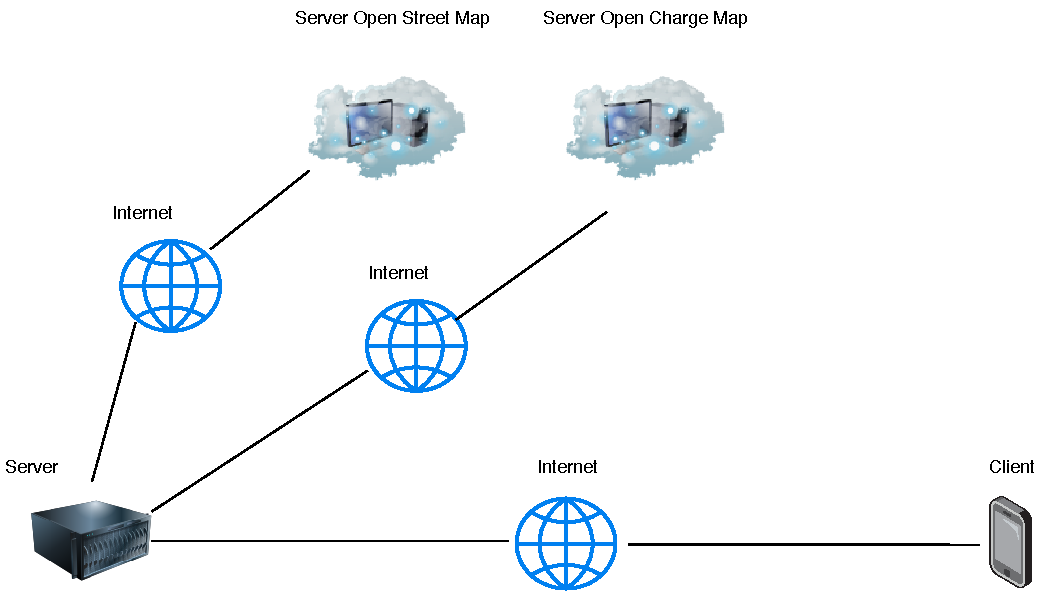
\includegraphics[scale=0.6]{Immagini/Architectural_Diagram.pdf}}
\caption{Architectural Diagram}
\end{figure}

\begin{figure}[htp]
\centering
{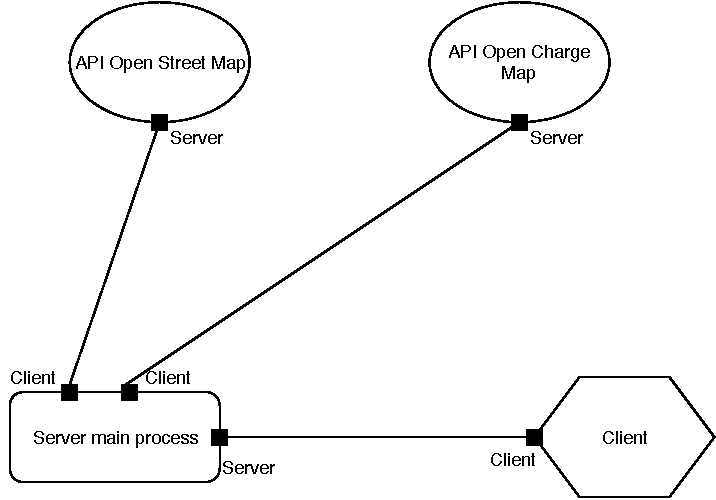
\includegraphics[scale=0.7]{Immagini/ClientServerArchitecture.pdf}}
\caption{Client-Server Architecture}
\end{figure}

\newpage

\section{Architettura Software}
L'archiettura software si divide in due diagrammi Component Diagram e Class Diagram.

\subsection{Component Diagram} \hypertarget{section::\theHsection}
Il diagramma delle componenti ha lo scopo di rappresentare la struttura interna del sistema software modellato in termini dei suoi componenti principali e delle relazioni fra di essi. (Figura 5.4)

\begin{figure}[htp]
\centering
{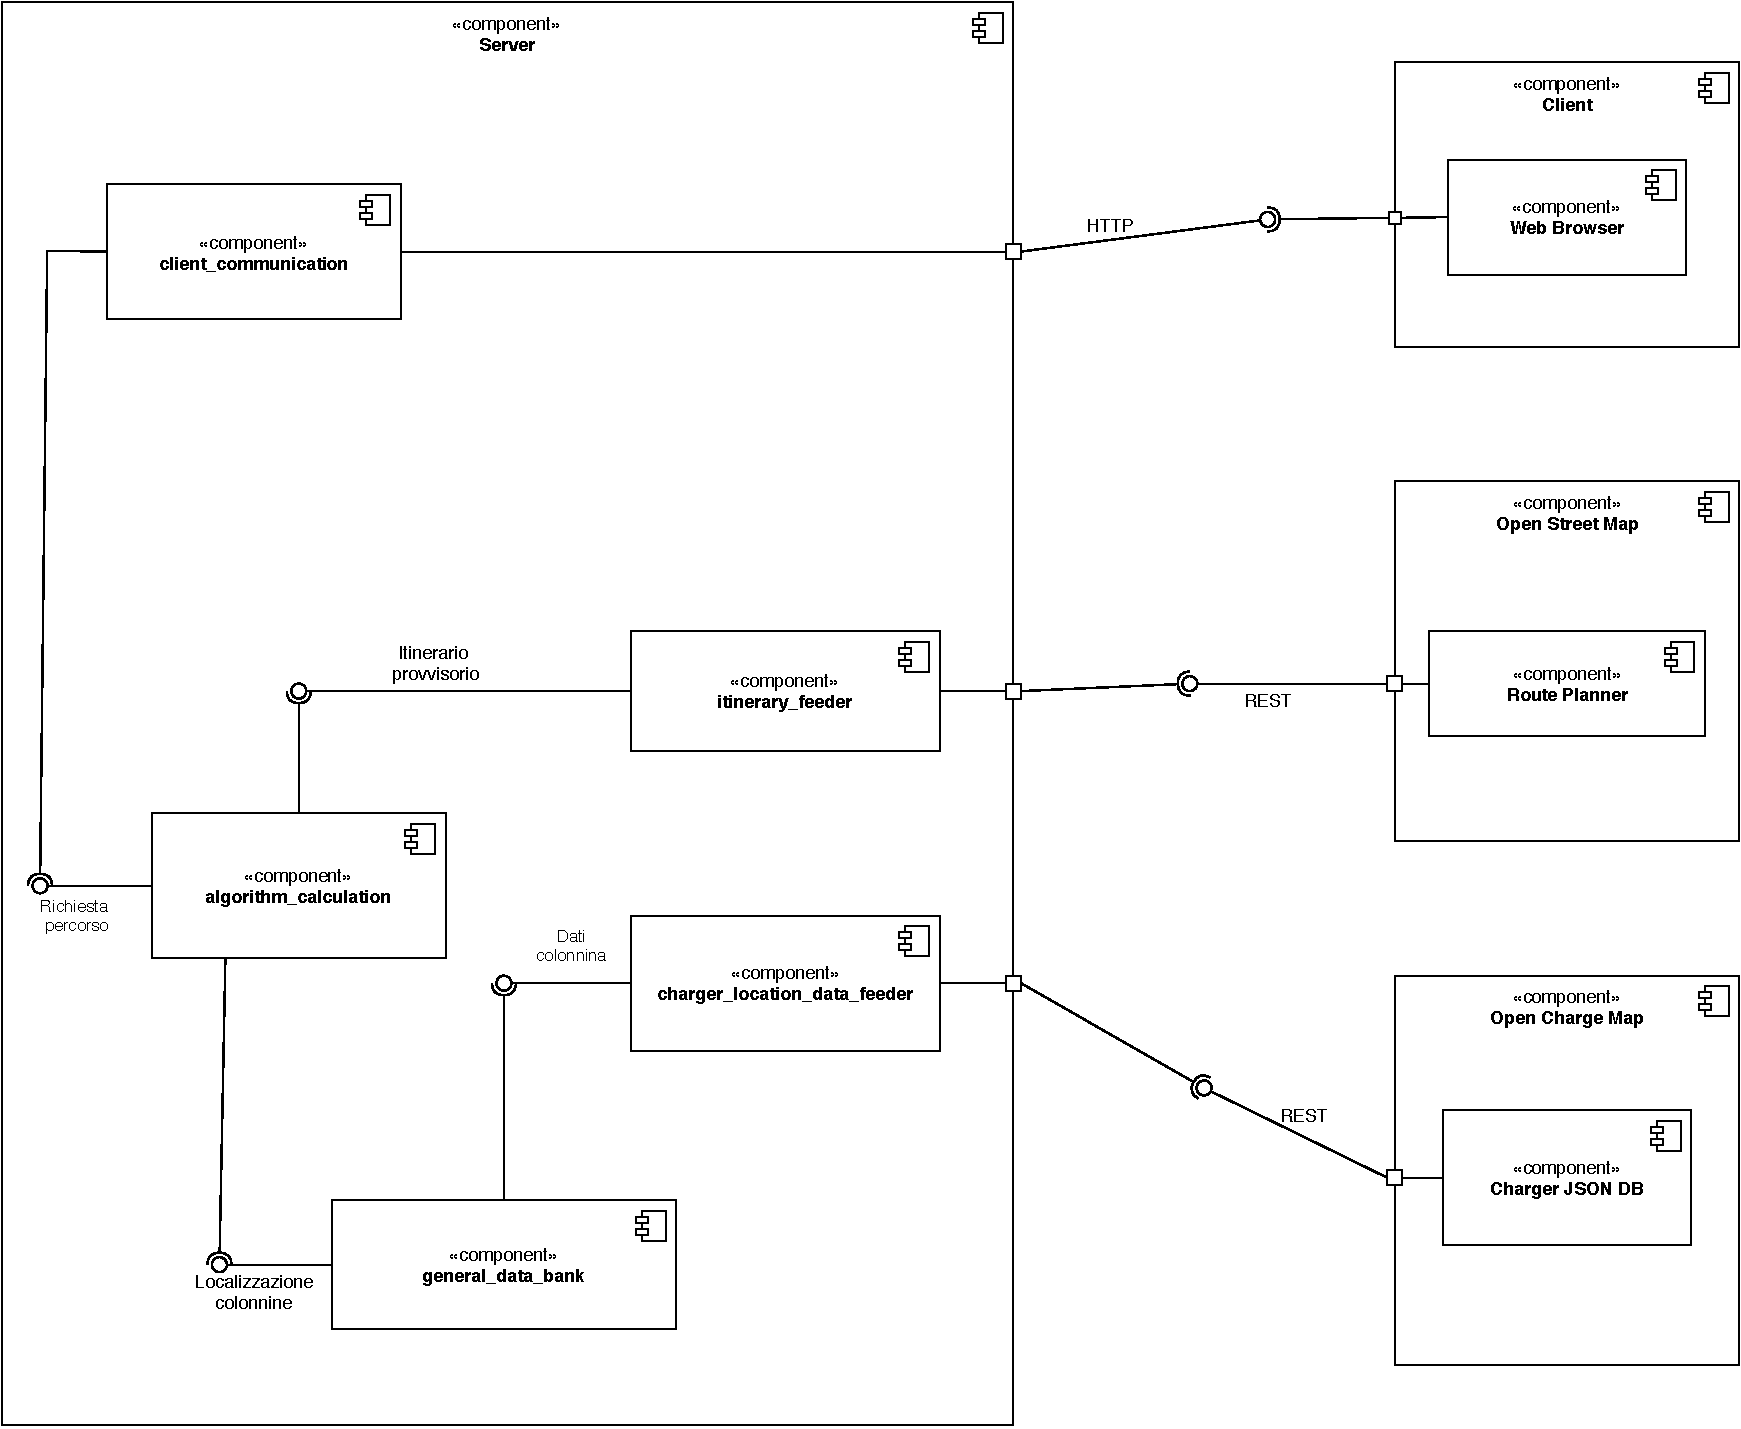
\includegraphics[scale=0.5]{Immagini/Component_Diagram.pdf}}
\caption{Component Diagram}
\end{figure}


\subsection{Class Diagram}
\hypertarget{section::\theHsection}
Il diagramma delle classi descrive il tipo degli oggetti che compongono il sistema e le relazioni statiche esistenti tra loro. (Figura 5.5)

\begin{figure}[htp]
\centering
{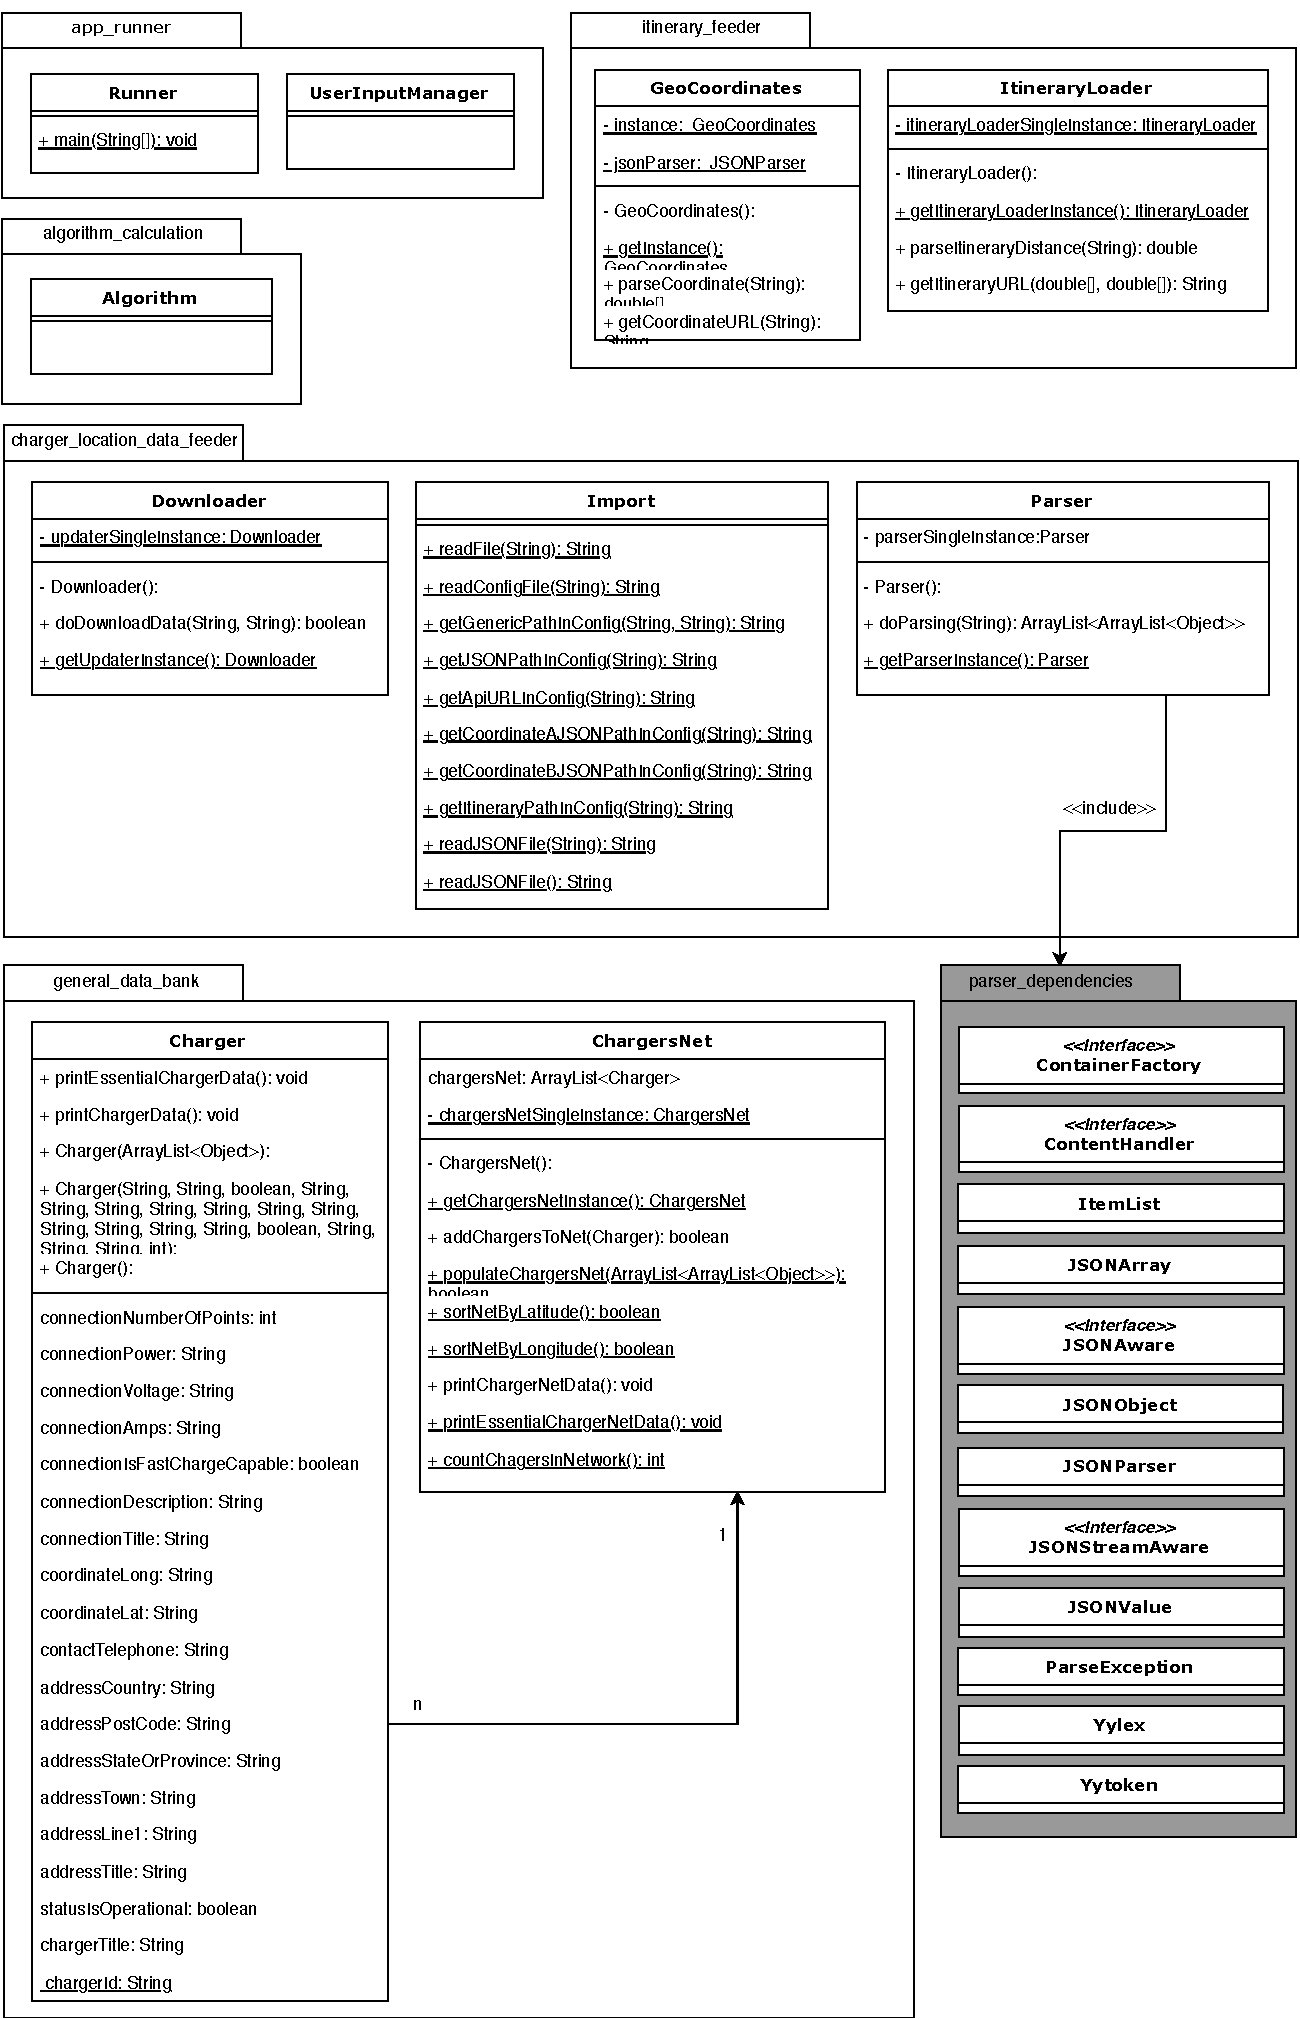
\includegraphics[scale=0.6]{Immagini/Class_Diagram.pdf}}
\caption{Class Diagram Architecture}
\end{figure}

\autocite[\protect\label{FerrariPighizzini2008}][]{FerrariPighizzini2008}